
\label{sec:two-fluid}

%We consider a system made of two phases, $\Omega_1(t)$ and $\Omega_2(t)$, separated by a sharp interface $\Sigma$(t), that fill the considered domain $\Omega \subset \mathbb{R}^3$, in such a way that $\Omega = \Sigma(t) \cup \Omega_1(t) \cup \Omega_2(t)$ (see \ref{fig:Scheme}). 
We consider a system made of two phases, \JL{1 and 2 (evite au maximum le verbiage mathematique qui n'apporte rien en physique)}, separated by a sharp interface $\Sigma$. Each phase subdomain is denoted $\Omega_1$ and $\Omega_2$ (see \ref{fig:Scheme}). These domains obey the physical and mathematical constraints defined in \cite{bothe2022sharp}. 
\JL{je ne vois pas bien ce que vient faire le papier de D. Bothe à ce stade ...} 
%These domains obey the physical and mathematical constraints defined in \cite{bothe2022sharp}. 
To track the position of the phase indexed $k$, we introduce the Phase Indicator Function (PIF), 
\begin{equation}
    \chi_k(\textbf{y},t) =  \left\{
      \begin{tabular}{cc}
        $1 \;\text{if} \;\textbf{y} \in \Omega_k(t)$\\
        $0 \;\text{if} \;\textbf{y} \notin \Omega_k(t)$
      \end{tabular}
      \right.
      \text{for $k = 1,2$}
      \label{eq:PIF}
\end{equation}
\begin{figure}[h!]
    \centering
    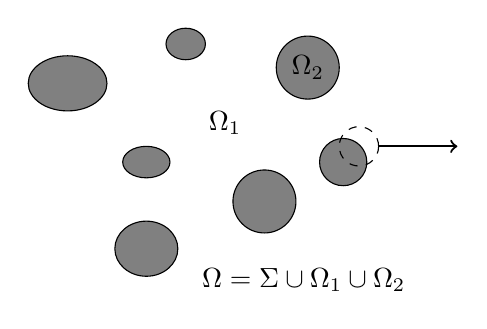
\begin{tikzpicture}
        \foreach \x/\y/\ra/\r in {
        1/3/0.2/0.25,
        2.55/2.7/0.4/0.4,
        0.5/0.4/0.35/0.4,
        2/1/0.4/0.4,
        3/1.5/0.3/0.3,
        0.5/1.5/0.2/0.3,
        -0.5/2.5/0.35/0.5}{
            \draw[fill=gray](\x,\y) ellipse(\r cm and \ra cm);
        }
        \draw[dashed](3.2,1.7)circle(0.25);
        % \draw[thick,->](3.2,1.7)++(0.1767,0.1767)--++(0.4,0.4)--++(1,0);
        \draw[thick,->](3.2,1.7)++(0.25,0)--++(1,0);
        \draw(2.55,2.7)node{$\Omega_2$};
        \draw(1.5,2)node{$\Omega_1$};
        \draw(2.5,0)node{$\Omega = \Sigma \cup \Omega_1 \cup \Omega_2$};
        % \draw(2.5,-1)node{$\Sigma = \sum_\alpha \Sigma_\alpha$};
        % \draw(2.5,-0.5)node{$\Omega_2 = \sum_\alpha \Omega_\alpha$};
    \end{tikzpicture}
    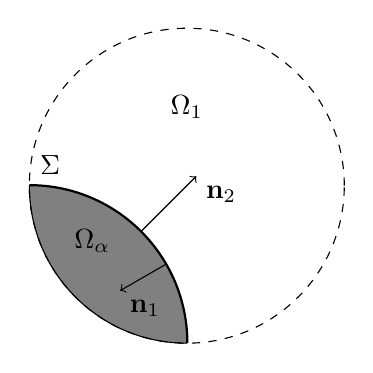
\begin{tikzpicture}%[scale = 0.9]
        \draw[very thick](0:2)arc(0:90:2)node[above right]{$\Sigma$};
        \draw[fill=gray](0:2)arc(0:90:2)arc(180:270:2);
        \draw[dashed](2,2)circle(2);
        \draw[->](1.42,1.42)--++(0.7,0.7)node[below right]{$\textbf{n}_2$};
        \draw[->](1.73,1)--++(-0.577,-0.333)node[below right]{$\textbf{n}_1$};
        \draw(2,3)node{$\Omega_1$};
        \draw(0.8,1.3)node{$\Omega_\alpha$};
    \end{tikzpicture}
    \caption{Scheme of the topology of dispersed two phase flows.}
    \label{fig:Scheme}
\end{figure}
From this point we drop the time and position arguments in the PIF. 

\subsection{Topological equations}
%By considering that the convective derivative of $\chi_k$ is zero at the interface points we can deduce that the transport equation of the $\chi_k$ reads 

Using the distribution formalism, one may show that the transport equation of $\chi_k$ reads\citep{drew1983mathematical} \JL{tu cites plein de papier en plus de Drew, mais cela n’est pas necessaire. Il faut juste citer la reference originelle}%,kataoka1986local,morel2015mathematical},
\begin{equation}
    \pddt \chi_k
    + \textbf{u}_I \cdot \nablabh \chi_k
    = 0,
    \label{eq:dt_chi_k}
\end{equation}
where $\textbf{u}_I$ is the velocity of the interface $\Sigma(t)$.
Additionally, it can be shown \citep{tryggvason2011direct,drew1983mathematical,kataoka1986local,bothe2022sharp} \JL{tu cites plein de papier en plus de Drew, mais cela n’est pas necessaire. Il faut juste citer la reference originelle} that,
\begin{equation}
    \nablabh \chi_k
    = - \delta_I \textbf{n}_k
    \label{eq:grad_chi_k}
\end{equation}
\JL{es tu sur du signe ?}
where we introduced the Interface Indicator Function (IIF) defined as $\delta_I = \delta(\textbf{y}-\textbf{y}_I)$ with $\delta$ \JL{is} the Dirac-delta function and $\textbf{y}_I$ the position vector lying on the domain $\Sigma(t)$ \JL{and $\textbf{y}_I$ the position of the interface}.
Besides, $\textbf{n}_k$ is defined as the outward normal vector of the domain $\Omega_k$ (see \ref{fig:Scheme}).
To describe the evolution of $\delta_I$ we take the gradient of \ref{eq:dt_chi_k} which yields \JL{reference ?}%the IIF transport equation,
\begin{equation}
    \pddt \delta_I
    + \nablabh \cdot \left[(\textbf{u}_I\cdot\textbf{n})\textbf{n} \delta_I\right]
    = \delta_I (\textbf{u}_I\cdot\textbf{n})(\nablabh \cdot\textbf{n}). 
\end{equation}
As pointed out by \citet{morel2007surface}, it is more convenient to rewrite this equation under the following form,
\begin{equation}
    \pddt \delta_I
    + \nablabh \cdot (\delta_I \textbf{u}_I)
    = \delta_I \nablabhI \cdot \textbf{u}_I.
    \label{eq:dt_delta_I}
\end{equation}
where we introduced the surface divergence operator defined as $\nablabhI \cdot ()= (\textbf{I}-\textbf{nn})\cdot \nablabh \cdot ()$ which is the \JL{surface} divergence operator \JL{la notation $\nablabhI$ n’est pas res heureuse, pq ne pas utiliser $\nabla _s$ comme tout le monde}

%projected on the tangential plan of $\Sigma(t)$. 
All along this work we \JL{make use of the subscript $_s$ to denote a quantity projected along the interface} such that $\textbf{f}_{s} = (\textbf{I}-\textbf{nn})\cdot \textbf{f}$ where $f$ is an arbitrary quantity \JL{mais f est une quantite arbitraire mais a quelle phase appartient elle ? est on oblige de definir cela maintenant ?}. for any arbitrary tensor $\textbf{F}$. \JL{We also} use the subscript $_I$ to denote any quantity belonging to $\Sigma$.   
Lastly, we can derive an expression for the gradient of $\delta_I$ by taking the gradient of \ref{eq:grad_delta_I} yielding \JL{tu cites lequation 6 que tu definis juste en dessous},
\begin{equation}
    \nablabh\delta_I 
    = \textbf{n} \cdot \nablabh (\textbf{n} \delta_I).
    \label{eq:grad_delta_I}
\end{equation}
Then, \ref{eq:dt_chi_k},\ref{eq:grad_chi_k}\ref{eq:dt_delta_I} and \ref{eq:grad_delta_I} \JL{repetition d'Equation a modifier} form the so-called topological equations for two phase flows. %which describe the local geometry of the flow.

\subsection{Local conservation equations}


Let $f_k(\textbf{y},t)$ being a volumetric quantity of arbitrary tensorial order defined in \JL{the k phase}%$\Omega_k(t)$.


%an arbitrary volumetric property
Likewise, let $f_I(\textbf{y},I)$ be an arbitrary surface property defined on $\Sigma(t)$ of arbitrary tensorial order.
Then it is possible to derive the local conservation equations for both volumetric and surface quantities following the strategy of \citep{bothe2022sharp,morel2015mathematical,tignol1986modelisation,marle1982macroscopic} \JL{est ce necessaire de citer tout ces papiers. D'ailleurs as tu regarde le papier de Gatignol ? je ne pense pas que ce soit l'objet du papier}.
Indeed, using Reynolds transport theorem \JL{a definir} and divergence theorem on an arbitrary small control volume we eventually find, \JL{ne serait il pas plus simple de dire:We assume $f_k(y, t)$ and ... obey the following conservation laws }
\begin{align}
    \label{eq:dt_f_k}
    \pddt f_k
    &= \nablabh \cdot \left(
        \mathbf{\Phi}_k
        - f_k\textbf{u}_k
        \right)
    + \textbf{S}_k
    & \text{ in } \Omega_k,&\\
    \pddt f_I  
    &= 
    \nablabhI \cdot (\mathbf{\Phi}_{I||} - f_I \textbf{u}_I)
    + \textbf{S}_I
    - \Jump{
        f_k (\textbf{u}_I - \textbf{u}_k)
        + \mathbf{\Phi}_k
     } 
    & \text{ on } \Sigma,&
    \label{eq:dt_f_I}
\end{align}
which are respectively the conservation equations of $f_k$ and $f_I$.
In \ref{eq:dt_f_I} we introduced the notation $\Jump{}$ which indicate the sum over both phases, i.e. $\Jump{} = \sum_{k=1}^2 [\ldots] \cdot \textbf{n}_k$ \JL{a on vraiment besoin de definir cette notation. Je trouve le signe $\sum$ plus claire}. 
 \JL{We defined defined different de define. pas de passe ici ! plus ce nest pas une definition mais une "conséquence" des equations definies ci-dessus.} $\mathbf{\Phi}_k$ and $\mathbf{\Phi}_I$ are the non-conservative flux tensors corresponding to $f_k$ and $f_I$. \JL{non-conservative ??? non-convective plutot. relis toi !}
The non-convective flux are often expressed through a constitutive equation depending on the nature of the flow such as the stress tensor for the momentum. \JL{pas claire : le tenseur
des contraintes est simplement l’expression du flux non convectif dans le
lequation de qdm. Les lois constitutives n’apparaissent que pour exprimer
par exemple la contrainte en fonction des grandeurs resolues}
$\textbf{S}_k$ and $\textbf{S}_I$ are respectively the volumetric and surface source terms.% on respectively, the domains $\Omega_k$ and $\Sigma$. 
Lastly, $\textbf{u}_k$ corresponds to the velocity fields defined in $\Omega_k$. 
It is important to notice that \ref{eq:dt_f_k} and \ref{eq:dt_f_I} are solely defined in respectively, $\Omega_k$ and $\Sigma$, therefore these equations are referred to, as local conservation equations.

\subsubsection*{Global conservation equations}

To generalize \ref{eq:dt_f_k} and \ref{eq:dt_f_I} over $\Omega$, we follow the method of \citet{drew1983mathematical} and \citet{kataoka1986local} for the volumetric equation, and \citet{marle1982macroscopic} for the surface equation.
Indeed, to any local quantities $f_k$ defined in $\Omega_k$, we assign the field $\chi_k f_k$ which is defined over the whole domain $\Omega$. 
Likewise, for any surface property $f_I$ defined on $\Sigma$, we assign the field quantity $\delta_I f_I$ which is also defined all over $\Omega$. 
Then, multiplying \ref{eq:dt_f_k} and \ref{eq:dt_f_I} by respectively $\chi_k$ and $\delta_I$, and making use of \ref{eq:dt_chi_k}, \ref{eq:dt_delta_I} and \ref{eq:grad_delta_I} gives, 
\begin{align}
    \pddt (\chi_k f_k)
    &= \nablabh \cdot (\chi_k \mathbf{\Phi}_k - \chi_k f_k \textbf{u}_k)
    + \chi_k \textbf{S}_k
    + \delta_I\left[
        \mathbf{\Phi}_k
        + f_k
        \left(
            \textbf{u}_I
            - \textbf{u}_k
        \right)
    \right]
    \cdot \textbf{n}_k ,
    % & \forall \textbf{y} \in \Omega&
    \label{eq:dt_chi_k_f_k}\\
    \pddt (\delta_If_I)  
    &= 
    \nablabh \cdot (\delta_I \mathbf{\Phi}_{I||} - \delta_I f_I \textbf{u}_I)
    +\delta_I\textbf{S}_I 
    - \delta_I \Jump{
    f_k (\textbf{u}_I - \textbf{u}_k)
    + \mathbf{\Phi}_k
    }.
    \label{eq:dt_delta_I_f_I}
\end{align}
which is respectively the volume and surface conservation of $\chi_kf_k$ and $\delta_If_I$. 
The set of equations formed by \ref{eq:dt_chi_k_f_k} for $k =1,2$ is commonly known as the \textit{two-fluid} formulation of multiphase flows, to which we add the \textit{jump condition} across the phase given by \ref{eq:dt_delta_I_f_I} \citep{morel2015mathematical,tryggvason2011direct,drew1983mathematical,kataoka1986local}. 
In this work, we prefer to think of those equations as a set of three equations formed by \ref{eq:dt_chi_k_f_k} and \ref{eq:dt_delta_I_f_I}. 
Indeed, if we define the \textit{bulk} property $f$ such as $f = \sum_k \chi_k f_k + \delta_I f_I$.
Then by adding \ref{eq:dt_chi_k_f_k} for $k=1,2$ and \ref{eq:dt_delta_I_f_I} gives the \textit{single-fluid} formulation,
\begin{equation}
    \pddt f
    = \nablabh \cdot (\mathbf{\Phi} - f \textbf{u})
    + \textbf{S},
    \label{eq:dt_f}
\end{equation}
Remark that we rather define \textit{bulk} quantities as $f = \sum_k \chi_k f_k$ and consider the interfacial component as a source term \citep{morel2015mathematical,tryggvason2011direct,drew1983mathematical}. 
Nevertheless, it is more practical to consider 3 phases flows variable since we made no assumption on the interfacial conservation equation. 
